%
% LaTeX template at the Institute for Optical Systems (IOS)
%
% Author: Nico Brügel  (nico.bruegel@htwg-konstanz.de)
% Date: 11.10.2019
%

% Include header
% !TEX root = ../thesis.tex
\documentclass[11pt,a4paper,oneside]{report}		                     

% Mathe
\usepackage{marvosym}		% Package für Euro&Co.
\usepackage{amsfonts}		% Package für Mengensymbole (IN, IR, ...)
\usepackage{amsmath}		% Package für restlichen Mathekram
\usepackage{amssymb}        % math. Symbole und Umgebungen
\usepackage{mathtools}
\usepackage{unicode-math}   % Erlaubt die Mathe Schrift zu setzen

% Use german umlaute
%\usepackage{ngerman}
\usepackage[ngerman]{babel}
%\usepackage[T1]{fontenc}
%\usepackage[utf8]{inputenc}
%\usepackage[english]{babel}

% Zitierung und Literaturverzeichnis
\usepackage{cite}
%\usepackage{apacite}		% Zitierstil
%\usepackage{natbib} 		% Erweiterte zitiermöglichkeiten 
\usepackage{babelbib}		% Übersetzung des Literaturverzeichnisses und der Zitate

% Fonts
\usepackage{fontspec}
\setmainfont[Path=fonts/, BoldFont=swis721-Bold.ttf, ItalicFont=swis721-Italic.ttf, BoldItalicFont=swis721-Bold-Italic.ttf]{swis721.ttf}
\setmonofont[Path=fonts/, BoldFont=CourierNew-Bold.ttf, ItalicFont=CourierNew-Italic.ttf, BoldItalicFont=CourierNew-Bold-Italic.ttf]{CourierNew.ttf}
\setmathfont[Path=fonts/]{CambriaMath.ttf}


% formatting
\usepackage{a4}

% PDF als Cover Hintergrund
\usepackage[firstpage=true]{background}
\usepackage{geometry}
\usepackage{tikz}

% Verbesserte Darstellug der Schriftzeichen und Zwischenräumen
%\usepackage{lmodern}				% Benutze skalierbare Schriftfamilie
%\usepackage[activate]{microtype}

% Heading styles
\usepackage[sf,bf,raggedright]{titlesec}
\titlespacing*{\section}
{0pt}{5.5ex plus 1ex minus .2ex}{4.3ex plus .2ex}
\titlespacing*{\subsection}
{0pt}{5.5ex plus 1ex minus .2ex}{4.3ex plus .2ex}
\titleformat{\chapter}[hang]{\Huge\bfseries}{\thechapter}{15pt}{\Huge\bfseries}

% Header and Footer
\usepackage{fancyhdr}

\fancypagestyle{fancybody}{
	\fancyhf{}
	\fancyhead[L]{\nouppercase{\leftmark}}
	\fancyfoot[C]{\thepage}
}

\fancypagestyle{plain}{
	\fancyhf{}
	\fancyfoot[C]{\thepage}
	\renewcommand{\headrulewidth}{0pt}
}

\pagestyle{fancybody}
\renewcommand{\chaptermark}[1]{\markboth{\normalfont\thechapter.\space#1}{}}

% Absatz einrücken unterdrücken
\setlength{\parindent}{0pt}

% Listings
\usepackage{listings}
\lstset{
	backgroundcolor=\color{lighter-gray},
	xleftmargin=\parindent,
	basicstyle=\ttfamily\footnotesize,
	breaklines=true,
	captionpos=b,
	showspaces=false,
	showstringspaces=false,
	frame=shadowbox,
	rulesepcolor=\color{ll-gray},
	rulecolor=\color{l-gray},
	belowskip=11pt,
}

% Depth of chapters and subsections
\setcounter{tocdepth}{3}
\setcounter{secnumdepth}{3}

% Url line break
\def\UrlBreaks{\do\/\do-}
\def\UrlBigBreaks{\do\:\do\/}

% Links
\usepackage[pdfstartview=FitV, 	% start in 'fit size height'-view
colorlinks=true, 	% Links farbig markieren
linkcolor=black, 	% Interne Links schwarz
citecolor=black, 	% Links zur Literatur schwarz
filecolor=black, 	% Links auf lokale Dateien schwarz
urlcolor=black,   	% Externe Links blau
breaklinks=true, 	% Links umbrechen
linktocpage=true 	% Im Inhaltsverzeichnis sind Seitenzahlen UND Text Links
]{hyperref}

%Move to the right.
\setlength{\hoffset}{5pt}
\setlength{\parskip}{\baselineskip}

% Suppress warning of too small headheight
\headheight13.6pt

% Abkuerzungsverzeichnis
\usepackage[nohyperlinks, printonlyused]{acronym}
\usepackage[mode=buildnew]{standalone}

\usepackage[toc, page]{appendix}


%%%%%%%%%%%%
%% HTWG CI Colors
%%%%%%%%%%%%
\definecolor{htwg-white}{cmyk}{0.0,0.0,0.0,0.0}
\definecolor{htwg-black}{cmyk}{0.0,0.0,0.0,1.0}
\definecolor{htwg-black-90}{cmyk}{0.0,0.0,0.0,0.9}
\definecolor{htwg-black-80}{cmyk}{0.0,0.0,0.0,0.8}
\definecolor{htwg-black-70}{cmyk}{0.0,0.0,0.0,0.7}
\definecolor{htwg-black-60}{cmyk}{0.0,0.0,0.0,0.6}
\definecolor{htwg-black-50}{cmyk}{0.0,0.0,0.0,0.5}
\definecolor{htwg-black-40}{cmyk}{0.0,0.0,0.0,0.4}
\definecolor{htwg-black-30}{cmyk}{0.0,0.0,0.0,0.3}
\definecolor{htwg-black-20}{cmyk}{0.0,0.0,0.0,0.2}
\definecolor{htwg-black-10}{cmyk}{0.0,0.0,0.0,0.1}
\definecolor{htwg-soft-blue}{cmyk}{0.1,0.0,0.0,0.1}
\definecolor{htwg-dark-blue}{rgb}{0.165, 0.22, 0.29}
\definecolor{htwg-teal}{cmyk}{1.0,0.0,0.5,0.0}


% Set variables used in cover, title, abstract and affidavit.
\newcommand{\ausgabedatum}{01.04.2020}
\newcommand{\abgabedatum}{30.06.2020}
\newcommand{\autor}{Lorenz Bung}
\newcommand{\autorStrasse}{Banater Str. 9}
\newcommand{\autorPLZ}{78467}
\newcommand{\autorOrt}{Konstanz}
\newcommand{\autorGeburtsort}{Konstanz}
\newcommand{\autorGeburtsdatum}{26.06.1997}
\newcommand{\prueferA}{Prof. Dr. Georg Umlauf}
\newcommand{\prueferB}{Simon Schmei{\ss}er}
\newcommand{\firma}{Isys Vision GmbH}
\newcommand{\studiengang}{Angewandte Informatik}


\newcommand{\thema}{Rekonstruktion von Meshes für industrielles Bin-Picking und Depalettieren}

\newcommand{\schlagworte}{Robotics, Geometric Modeling, Machine Vision, Mesh Reconstruction}

\begin{document}

% Include title pages
% !TEX root = ../thesis.tex
\begin{titlepage}

\vspace*{-2.5cm}

\begin{figure}[h]
\hspace*{-2cm}

\includegraphics[height=2cm]{title/HTWG-Logo_en_300dpi.png}
\hspace*{4cm}
\includegraphics[height=2cm,]{title/IOS_Logo2016_lettering_en.png}


\end{figure}

\vspace{2cm}

\begin{center}
	 \LARGE{
		\textbf{\thema} \\[5cm]
	}
	\Large{
		\textbf{\autor}} \\[5.5cm]
	\large{
		\textbf{Konstanz, \abgabedatum} \\[2.3cm]
	}
	
	\Huge{
		\textbf{{\sf BACHELORARBEIT}}
	}
\end{center}

\end{titlepage}

% !TEX root = ../thesis.tex
\thispagestyle{empty}
{
\setlength{\parskip}{1cm}
        \begin{center}
        \textbf{\Huge BACHELORARBEIT}\\[15ex]

        \textbf{zur Erlangung des akademischen Grades}

        \textbf{\Large Bachelor of Science (B. Sc.)}

        \textbf{an der}

        \textsf{\huge Hochschule Konstanz}\\
        {\small Technik, Wirtschaft und Gestaltung}

        \textsf{\Large Fakultät Informatik} \\
        Studiengang \studiengang\\[15ex]
        
        \begin{tabular}{p{3cm} p{7cm}}
        Thema: & \thema\\[1cm]
        Kandidat: & \autor \\
        	                  & \autorStrasse \\
                          & \autorPLZ\ \autorOrt \\[1cm]
        1. Prüfer: & \prueferA \\
        2. Prüfer: & \prueferB \\[1cm]
        Ausgabedatum: & \ausgabedatum \\
        Abgabedatum: & \abgabedatum \\
        \end{tabular}
        \end{center}
}

\newpage


% Set page numbering to roman
\pagenumbering{Roman}

% Include abstract and affidavit
% !TEX root = ../thesis.tex
\thispagestyle{plain}
\chapter*{Ehrenwörtliche Erklärung}
\label{ch:affidavit}

Hiermit erkläre ich,
\textit{\autor, geboren am \autorGeburtsdatum\ in \autorGeburtsort}, dass ich\\

\begin{tabular}{lp{12cm}}
(1) & meine Bachelorarbeit mit dem Titel \\[1em]
& \textbf{\thema} \\[1em]
& bei \firma\ unter Anleitung von \prueferA\ und \prueferB\ selbständig und ohne fremde Hilfe angefertigt und keine anderen als die angeführten Hilfen benutzt habe;\\[1em]
(2) & die Übernahme wörtlicher Zitate, von Tabellen, Zeichnungen, Bildern und
Programmen aus der Literatur oder anderen Quellen (Internet) sowie die Verwendung
der Gedanken anderer Autoren an den entsprechenden Stellen innerhalb der Arbeit
gekennzeichnet habe;\\[1em]
(3) & dass die eingereichten Abgabe-Exemplare in Papierform und im PDF-Format vollständig übereinstimmen.
\end{tabular}

\vspace*{1cm}

\noindent
Ich bin mir bewusst, dass eine falsche Erklärung rechtliche Folgen haben wird.\\

\vspace*{1cm}

\noindent
Konstanz, \abgabedatum \hfill \begin{tabular}{c} \\ \\ \rule{5cm}{1pt} \\ (Unterschrift)\end{tabular}

\newpage

% !TEX root = ../thesis.tex
\thispagestyle{plain}
\chapter*{Abstract}
\label{ch:abstract}


\begin{center}
	\begin{tabular}{p{3.2cm}p{9.6cm}}
		Thema: & \thema \\[1ex]
		% & \\
		Bachelorkandidat: & \autor \\[1ex]
		% & \\
		Betreuer: & \prueferA \\%[.5ex]
		 & Institut für Optische Systeme\\[1ex]
		 & \prueferB \\%[.5ex]
		 & \firma \\[1ex]
		% & \\
		Abgabedatum: & \abgabedatum \\[1ex]
		% & \\
		Schlagworte: & \schlagworte \\
		% & \\
	\end{tabular}
\end{center}


Describe the objective and results of this thesis in a few words.
Typically one page.

In dieser Arbeit werden verschiedene Ansätze zur Rekonstruktion von Meshes aus 3D-Punktwolken analysiert, miteinander verglichen und bewertet.
Die erste Methode ist YAK, eine Variante von Kinect Fusion, bei der ein Truncated Signed Distance Field zum Einsatz kommt.
Der zweite Ansatz ist, ein einzelnes Teil mithilfe einer beweglichen Kamera am Roboterarm aus mehreren Posen einzuscannen und so ein Gesamtbild zu erhalten.
Im dritten Ansatz wird eine 

\newpage

% !TEX root = ../thesis.tex
\thispagestyle{plain}
\chapter*{Extended Abstract}
\label{ch:extended-abstract}

\begin{refsection}

\begin{center}
	\begin{tabular}{p{3cm}p{10cm}}
		Thema: & \thema \\[1ex]
		Kandidat: & \autor \\[1ex]
		Betreuer: & \prueferA \\
		 & Institut für Optische Systeme\\[1ex]
		 & \prueferB \\
		 & \firma \\[1ex]
		Abgabedatum: & \abgabedatum \\[1ex]
		Schlagworte: & \schlagworte \\[1ex]
	\end{tabular}
\end{center}


\section*{Einleitung}

Robotik spielt im industriellen Bereich eine größer werdende Rolle.
Insbesondere das sogenannte Bin-Picking, also das autonome Greifen unsortierter Teile gewinnt zunehmend an Relevanz.
Zur Erkennung der Objekte werden dabei in vielen Fällen CAD-Modelle benötigt, welche jedoch nicht immer vorliegen.
Die Rekonstruktion aus aufgenommenen 3D-Daten bietet daher eine einfache Möglichkeit, diese zu erhalten.
Es wurden verschiedene Ansätze dafür analysiert, verglichen und bewertet.


\section*{Methodik}

Die Pipeline wurde in großen Teilen auf Basis der Point Cloud Library \cite{rusu2011pcl} implementiert.
Um größtmögliche Flexibilität zu erreichen, wurde das Robot Operating System \cite{quigley2009ros} für die Interaktion mit dem Programm eingesetzt.
Zur Aufnahme der 3D-Punktwolken wurden Kameras von Ensenso \cite{ensensoWebsite} verwendet.

Die Segmentierung der Punktwolke wurde sowohl im 3D durch Euclidean Cluster Extraction und Region Growing getestet, als auch im zweidimensionalen Grauwertbild mithilfe des Watershed-Algorithmus.

Um Punktwolken aneinander auszurichten, wurde zunächst eine globale Registrierung durch 4-Point Congruent Sets \cite{aiger2008fpcs} durchgeführt.
Diese wurde anschließend mit Iterative Closest Point \cite{besl1992method} lokal optimiert.

Zur Triangulierung wurde der Poisson-Algorithmus \cite{kazhdan2006poisson} verwendet. Anschließend wurden alle Faces aus dem Mesh entfernt, welche eine gewählte Distanz von der Punktwolke überschritten.


\section*{Ergebnisse}

Zur Evaluation wurde die Cloud-Mesh-Distanz zwischen den Vertices des generierten Meshs und den Faces des Referenzobjekts bestimmt.
Außerdem wurde die inverse Cloud-Mesh-Distanz errechnet, um die Vollständigkeit zu überprüfen.

\begin{figure}[H]
    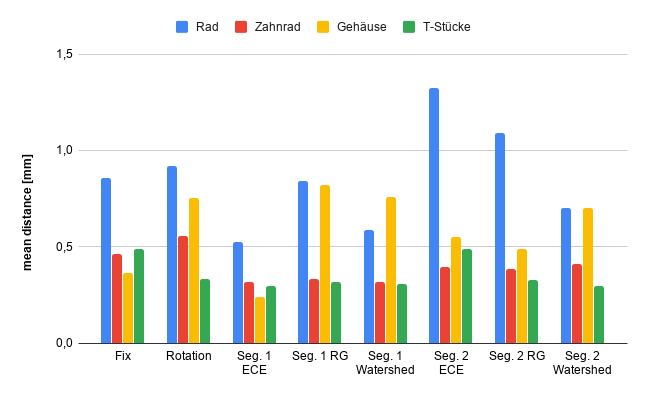
\includegraphics[width=0.49\textwidth]{images/segmentation/meanDistance1.png}
    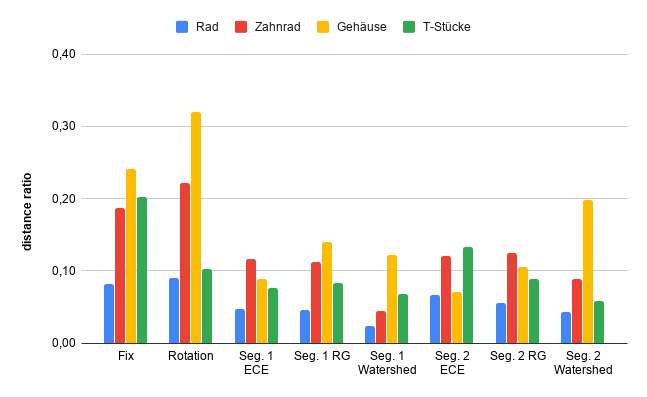
\includegraphics[width=0.49\textwidth]{images/segmentation/ratio.png}
    \caption{Cloud-Mesh-Distanz und Distanzverhältnis verschiedener Testobjekte}
    \label{fig:ex-abstract-distances}
\end{figure}

Es hat sich gezeigt, dass eine Rekonstruktion aus mehreren Aufnahmen eines einzelnen Objekts aus verschiedenen Perspektiven die höchste Qualität erreicht.
In \autoref{fig:ex-abstract-distances} sind die Cloud-Mesh-Distanz von Rekonstruktion zu Referenzobjekt sowie das Distanzverhältnis zu sehen.

Weiterhin ist aufgefallen, dass eine gute Rekonstruktion nur bei korrekter Segmentierung möglich ist.
Bei Untersegmentierung der Punktwolke müssen viele Cluster verworfen werden, während eine korrekte Registrierung bei einer Übersegmentierung oft nicht möglich ist.
Die Wahl der besten Segmentierungsmethode ist abhängig von der Objektform und -größe.

%TODO

\printbibliography[heading=subbibliography]

\end{refsection}
\newpage


% Include table of contents
\tableofcontents
\newpage

% Aktuelle Seitenzahl in einem Zähler speichern
% -> römische Seitennummerierung soll durchgängig
% sein und wird nachher wieder aufgegriffen.
% --------------------------------------------------------
\newcounter{anhang}
\setcounter{anhang}{\value{page}}

% Set page numbering to arabic
\pagenumbering{arabic}

% Include the chapters
% ---------------------------------------------------------------------------
\include{chapters/introduction}
\include{chapters/fundamentals}
\include{chapters/experiments}
\include{chapters/discussion-conclusion}

% ---------------------------------------------------------------------------
\pagenumbering{Roman}
\setcounter{page}{\value{anhang}}
% !TEX root = ../thesis.tex
\addcontentsline{toc}{chapter}{\bibname}
\bibliographystyle{ieeetr}
\bibliography{bib/references}
%\printbibliography[heading=bibintoc]
% Include appendix and lists if needed
%% !TEX root = ../thesis.tex
\addcontentsline{toc}{chapter}{List of Figures}
\listoffigures
%% !TEX root = ../thesis.tex
\addcontentsline{toc}{chapter}{List of Tables}
\listoftables
%% !TEX root = ../thesis.tex
\begin{appendices}

\chapter{Proofs}


\chapter{Additional Figures}

\chapter{Additional Table}


\end{appendices}

\end{document}
